\newcommand{\ProjectName}{LineaCasaBari}

\newcommand{\makeFrontPage}{
  % Declare new goemetry for the title page only.
  \newgeometry{top=3.5cm}
  
  \begin{titlepage}
  \begin{center}

  \begin{center}
  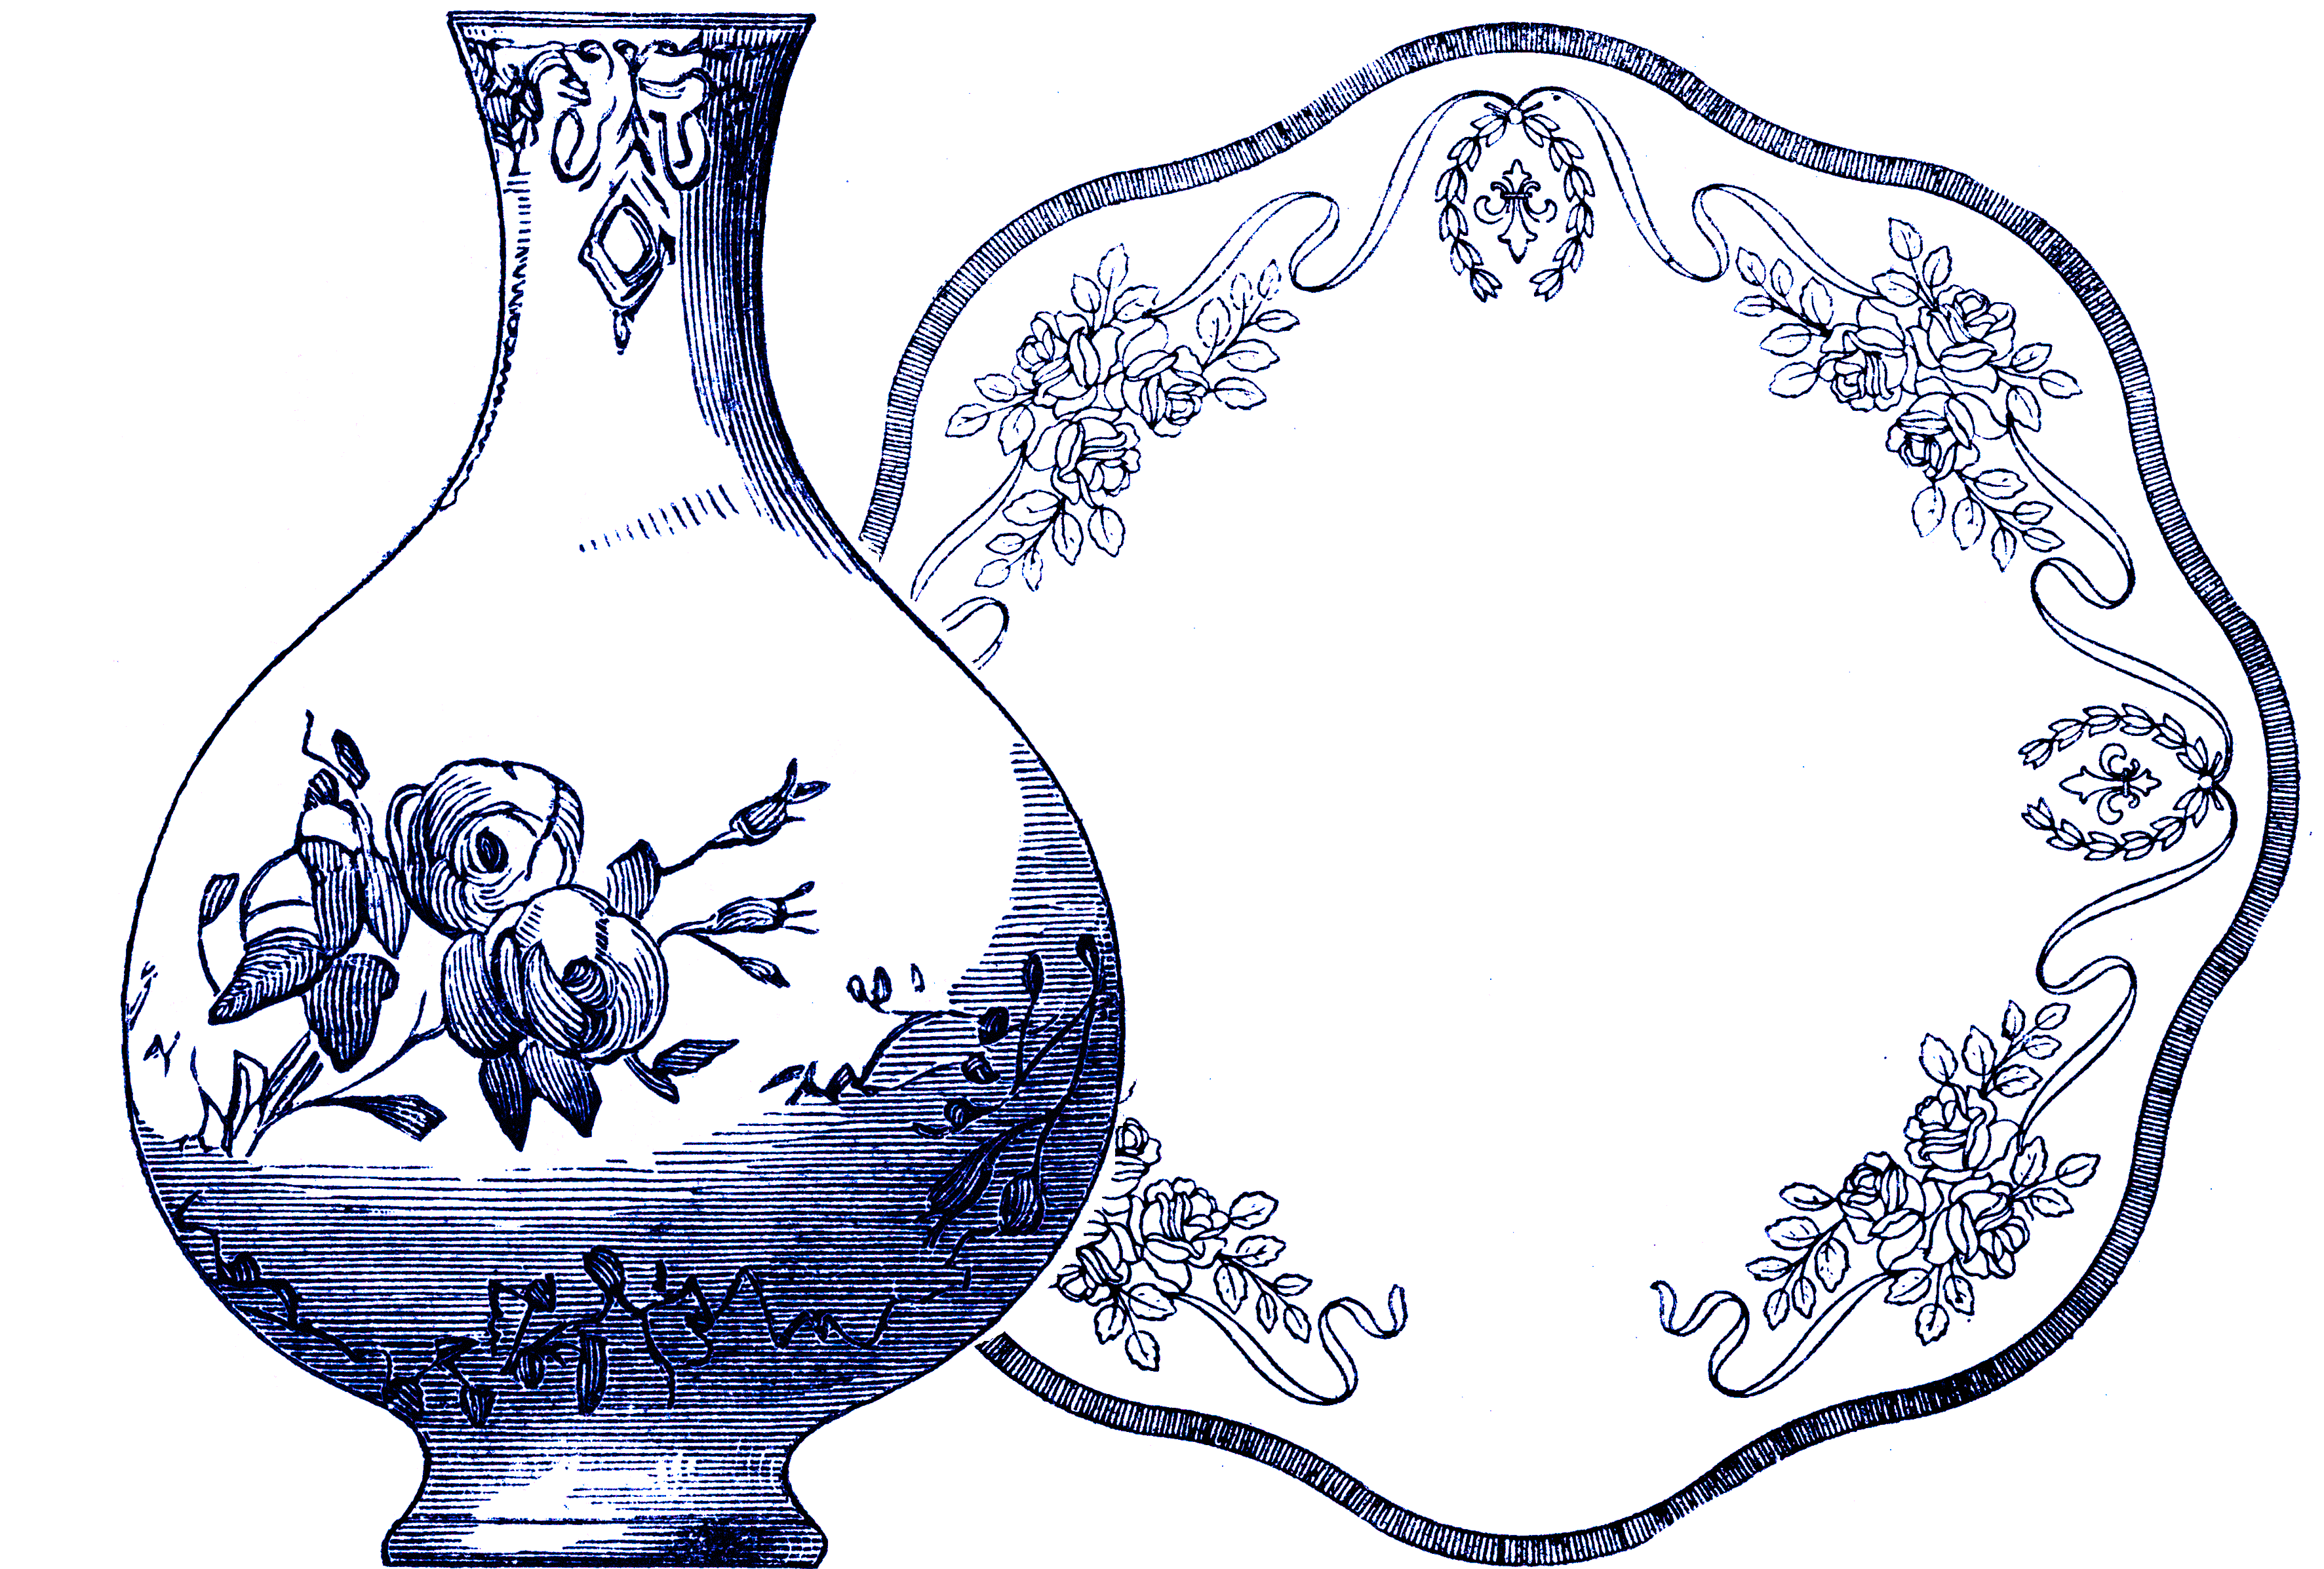
\includegraphics[width=10cm]{logo.png}
  \end{center}
  
  \vspace{1cm}

  \begin{Huge}
  \textbf{\ProjectName{}}
  \end{Huge}
  
  \vspace{11pt}

  \bgroup
  \def\arraystretch{1.3}
  \begin{tabular}{ r|l }
    \multicolumn{2}{c}{\textbf{Membri del gruppo}} \\
    \hline

    \textbf{Navid Taha} & 1069126 \\
    \textbf{Alice Sasso} & 1074588 \\
    \textbf{Lorenzo Ferrarin} & 1069405 \\
    \textbf{Alessandro Bari} & 1074356 \\
  \end{tabular}
  \egroup

  \vspace{22pt}

  \textbf{Informazioni sul sito} \\
  
  	\url{http://tecnologie-web.studenti.math.unipd.it/tecweb/~asasso/}
  	
  \vspace{5pt}
  \textbf{Referente} \\
  Navid Taha: navid.taha@studenti.unipd.it
  
  \vspace{7pt}  
  
  \textbf{Dati di accesso} \\
  
  
  
  login amministratore e utente
    
  
  \end{center}
  \end{titlepage}
  
  % Ends the declared geometry for the titlepage
  \restoregeometry
}